\section{Related Work: Multimodal Interaction}
\subsection{The Power of Speech}
In 2016, Google reported that 20\% of all search queries on mobile Android devices were spoken \cite{Pichai2016}; that number has likely grown. Speech input is especially appealing on mobile devices, as people often use them while on the go and busy with other tasks \cite{Guy2016}; but even on desktop computers, voice assistants are often used for web search \cite{Mehrotra2016}. Speaking a search query is often easier and faster than typing it out, and it allows the user to ask a question in the way they might ask a friend; mobile voice queries tend to be closer to natural language and more often phrased as questions than text queries \cite{Guy2016}. Also, people tend to search by voice more when seeking audio or video results \cite{Guy2016}, supporting ReMap's approach of using speech to search for videos. Finally, speech may be more useful for users with specific goals: Laput \textit{et al.} \cite{Laput2013} found that when editing photos, speech was most useful when people knew exactly what they wanted to do. When people didn't know what they wanted, browsing a gallery of examples was more helpful as it allowed them to compare visual previews of potential effects before choosing one. Therefore, ReMap's main intended use case is for situations where users have targeted questions in the middle of a task, as RePlay was found to be most helpful in such cases and speech is likely to be especially beneficial. In other words, ReMap supports users seeking procedural help for achieving a specific outcome.

\subsection{Combining Modalities can Maximize Cognitive Abilities}
Combining input from multiple modalities (\textit{e.g.}, speech, gesture, touch) can reduce cognitive load for complex tasks \cite{Oviatt2015, Reeves2004}, make tedious tasks more efficient \cite{Oviatt1999, Salisbury1990, Karl1993, Hugunin1997}, reduce errors \cite{Oviatt1999}, increase precision \cite{Cohen1989}, and even make tasks more enjoyable \cite{Oviatt1999, Laput2013}. Such combinations work best when they maximize users' working memory by using different modalities for different types of information \cite{Oviatt2015, Kalyuga1999, Reeves2004, Stanney2004}. 
%Auditory output is helpful for giving the user information while they work \cite{Stanney2004, Grossman2007, Reeves2004}, and visual output and manual input are helpful for conveying spatial information \cite{Stanney2004, Reeves2004}. 
For example, telling the user about keyboard shortcuts for the operations they execute via auditory feedback increases the likelihood that users will retain them, as users' auditory working memory is otherwise unused when working in software \cite{Grossman2007}. Similarly, using speech to navigate tutorial videos while one's hands are busy with a physical task allows users to process both the video and the task simultaneously \cite{Chang2019}. ReMap similarly partitions different modalities between the user's creative task and ReMap's help-seeking interface (\autoref{fig:remap_modalities}), allowing users to speak search queries and video navigation commands.

\begin{figure}[t]
\centering
  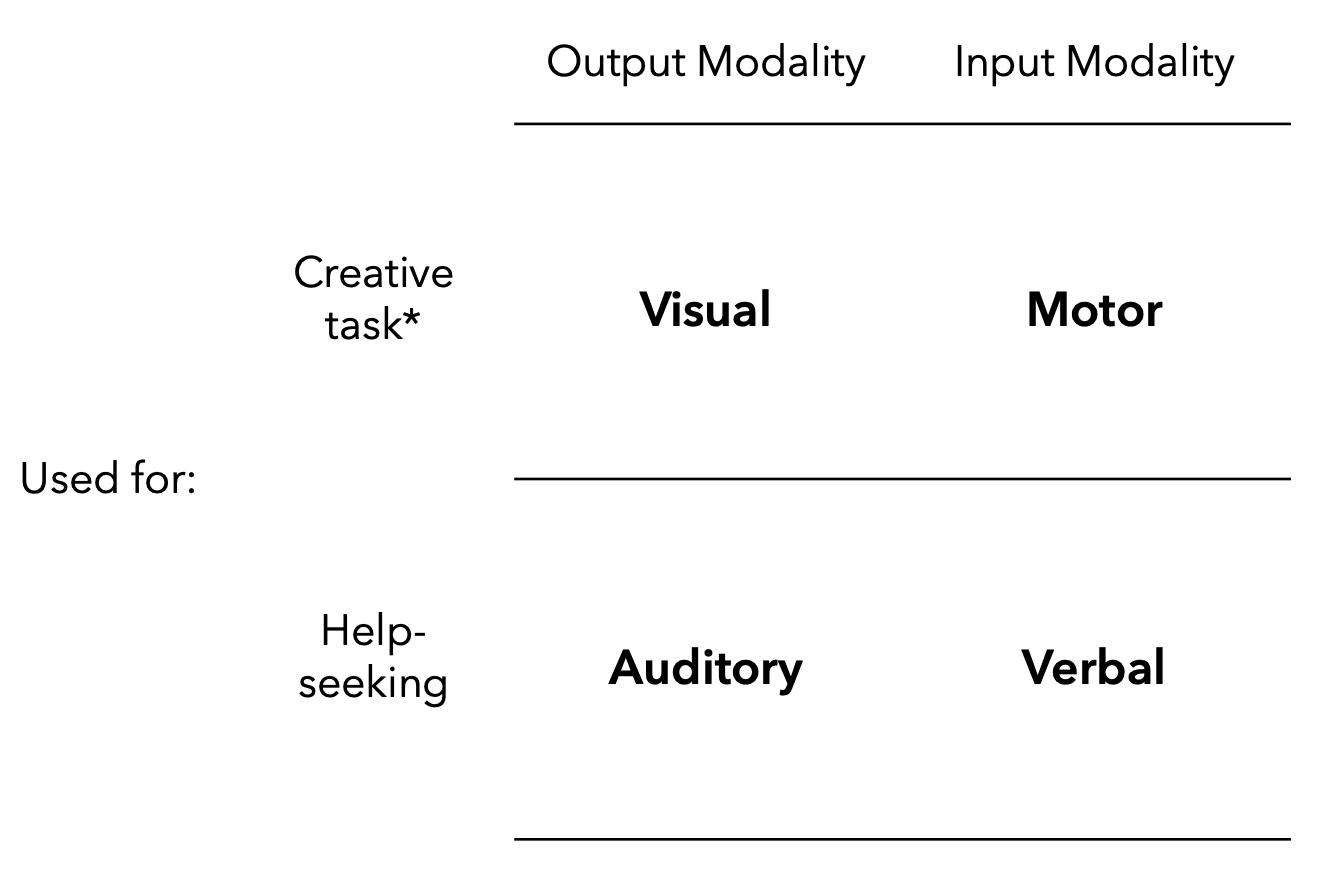
\includegraphics[width=0.7\textwidth]{remap/figures/remap_modalities.png}
  \caption[ReMap partitions the above modalities between the user's creative task and their help-seeking task to maximize cognitive abilities. Users primarily use speech and listening to search for and navigate help videos while keeping their hands and eyes on their creative task.]{ReMap partitions the above modalities between the user's creative task and their help-seeking task to maximize cognitive abilities. Users primarily use speech and listening to search for and navigate help videos while keeping their hands and eyes on their creative task. The * indicates that the visual and motor modalities are not \textit{exclusively} used for the creative task; users can also transfer their visual and motor attention to the help resources when necessary, \textit{e.g.}, to watch a video or type a search query manually.}~\label{fig:remap_modalities}
\end{figure}

Pointing at objects and spatial locations is often easier and more natural than describing them in words only \cite{Reeves2004, Bolt1980, Larkin1987}. Similarly, using a screenshot of an interface element as a search query is easier than describing it in text \cite{Yeh2009}. When combined with speech, pointing allows people to communicate more precisely by using deictic terms (\textit{e.g.,} ``this'', ``here'') to refer to objects and spatial locations while pointing at them \cite{Bolt1980, Laput2013}. ReMap similarly allows users to point at interface elements and canvas objects in their creative software and reference them deictically while speaking a search query.

Multimodal input can be especially beneficial for creative tasks, where maintaining a flow state is important. Using different modalities for software-related actions allows users to keep their focus and hands on their creative work. For example, using speech to access tools instead of menus or keyboard shortcuts can help artists maintain creative flow and stay focused on their task \cite{Kim2019, Sedivy1999}. While doing digital painting, an artist could switch from the brush tool to the eraser by saying ``eraser'' instead of switching their attention and moving their hands to the toolbar or keyboard \cite{Kim2019}. Not surprisingly, much prior work exploring multimodal input has centered around creative tasks such as photo editing \cite{Laput2013}, graphic design \cite{Kim2019}, drawing \cite{Sedivy1999, Pausch1991}, data visualization \cite{Setlur2016}, and 3D modeling \cite{Sharma2011}. However, most of this prior work has used speech to execute commands, rather than issue search queries. This requires either defining a list of acceptable commands (which users must then memorize) or parsing natural language commands (which is prone to errors). This chapter combines insights from multimodal creative systems and voice search systems to explore how using voice to search might be useful in creative software.
